\documentclass[a4paper, 12pt]{report}
\usepackage{graphicx} % Required for inserting images
\usepackage[T1]{fontenc}
\usepackage[latin1]{inputenc}
\usepackage{glossaries}
\usepackage{graphicx}
\usepackage{amsfonts}
\usepackage{subfigure}
\usepackage[hidelinks]{hyperref}
\usepackage{pifont}
\usepackage{array}

\usepackage{subcaption}

\usepackage{booktabs}
\usepackage{cleveref}
\usepackage{algorithm}
\usepackage{algpseudocode}
\usepackage{multicol}
\usepackage{eufrak}
\usepackage{amssymb}
\usepackage{listings}
\usepackage{amsthm}
\usepackage{verbatim}
\usepackage{tikz}
\usetikzlibrary{shapes,arrows}
\usepackage{tikz}
\tikzstyle{mybox} = [draw=black, thin, rectangle, rounded corners, inner ysep=5pt, inner xsep=5pt, fill=blue!15]
\newtheorem{theorem}{Teorema}
\usepackage[a4paper, top=2.8cm , bottom=2cm , right=2cm , left=2cm ]{geometry}

\usepackage[table,xcdraw]{xcolor}
\usepackage{array}
\usepackage{biblatex} %Imports biblatex package
\addbibresource{biblio_ROB.bib} %Import the bibliography file
\usepackage{longtable}
\usepackage{minitoc}
\usepackage{tabularx}   % Per colonne a larghezza variabile
\mtcsetdepth{minitoc}{1}
\usepackage{xcolor}
%\usepackage{newpxtext,newpxmath} %per stile palatino

\renewcommand{\mtctitle}{In this chapter we will see...}

\theoremstyle{definition}
\newtheorem{definition}{Definition}[section]

\pagestyle{headings}

\theoremstyle{remark}
\newtheorem*{remark}{Remark}

\begin{document}
\dominitoc
\newcommand{\bb}[1]{\mathbf{#1}}

\begin{titlepage}
    \centering
    
\includegraphics[width=0.35\textwidth]{img/logo_Polito_nuovo.png}\\[0.7cm] % Sostituisci con il nome del tuo file
    \vfill
    {\Huge \textbf{ROBOTICS}\\[1cm]
    \textit{Lecture notes}}\\[2cm]

    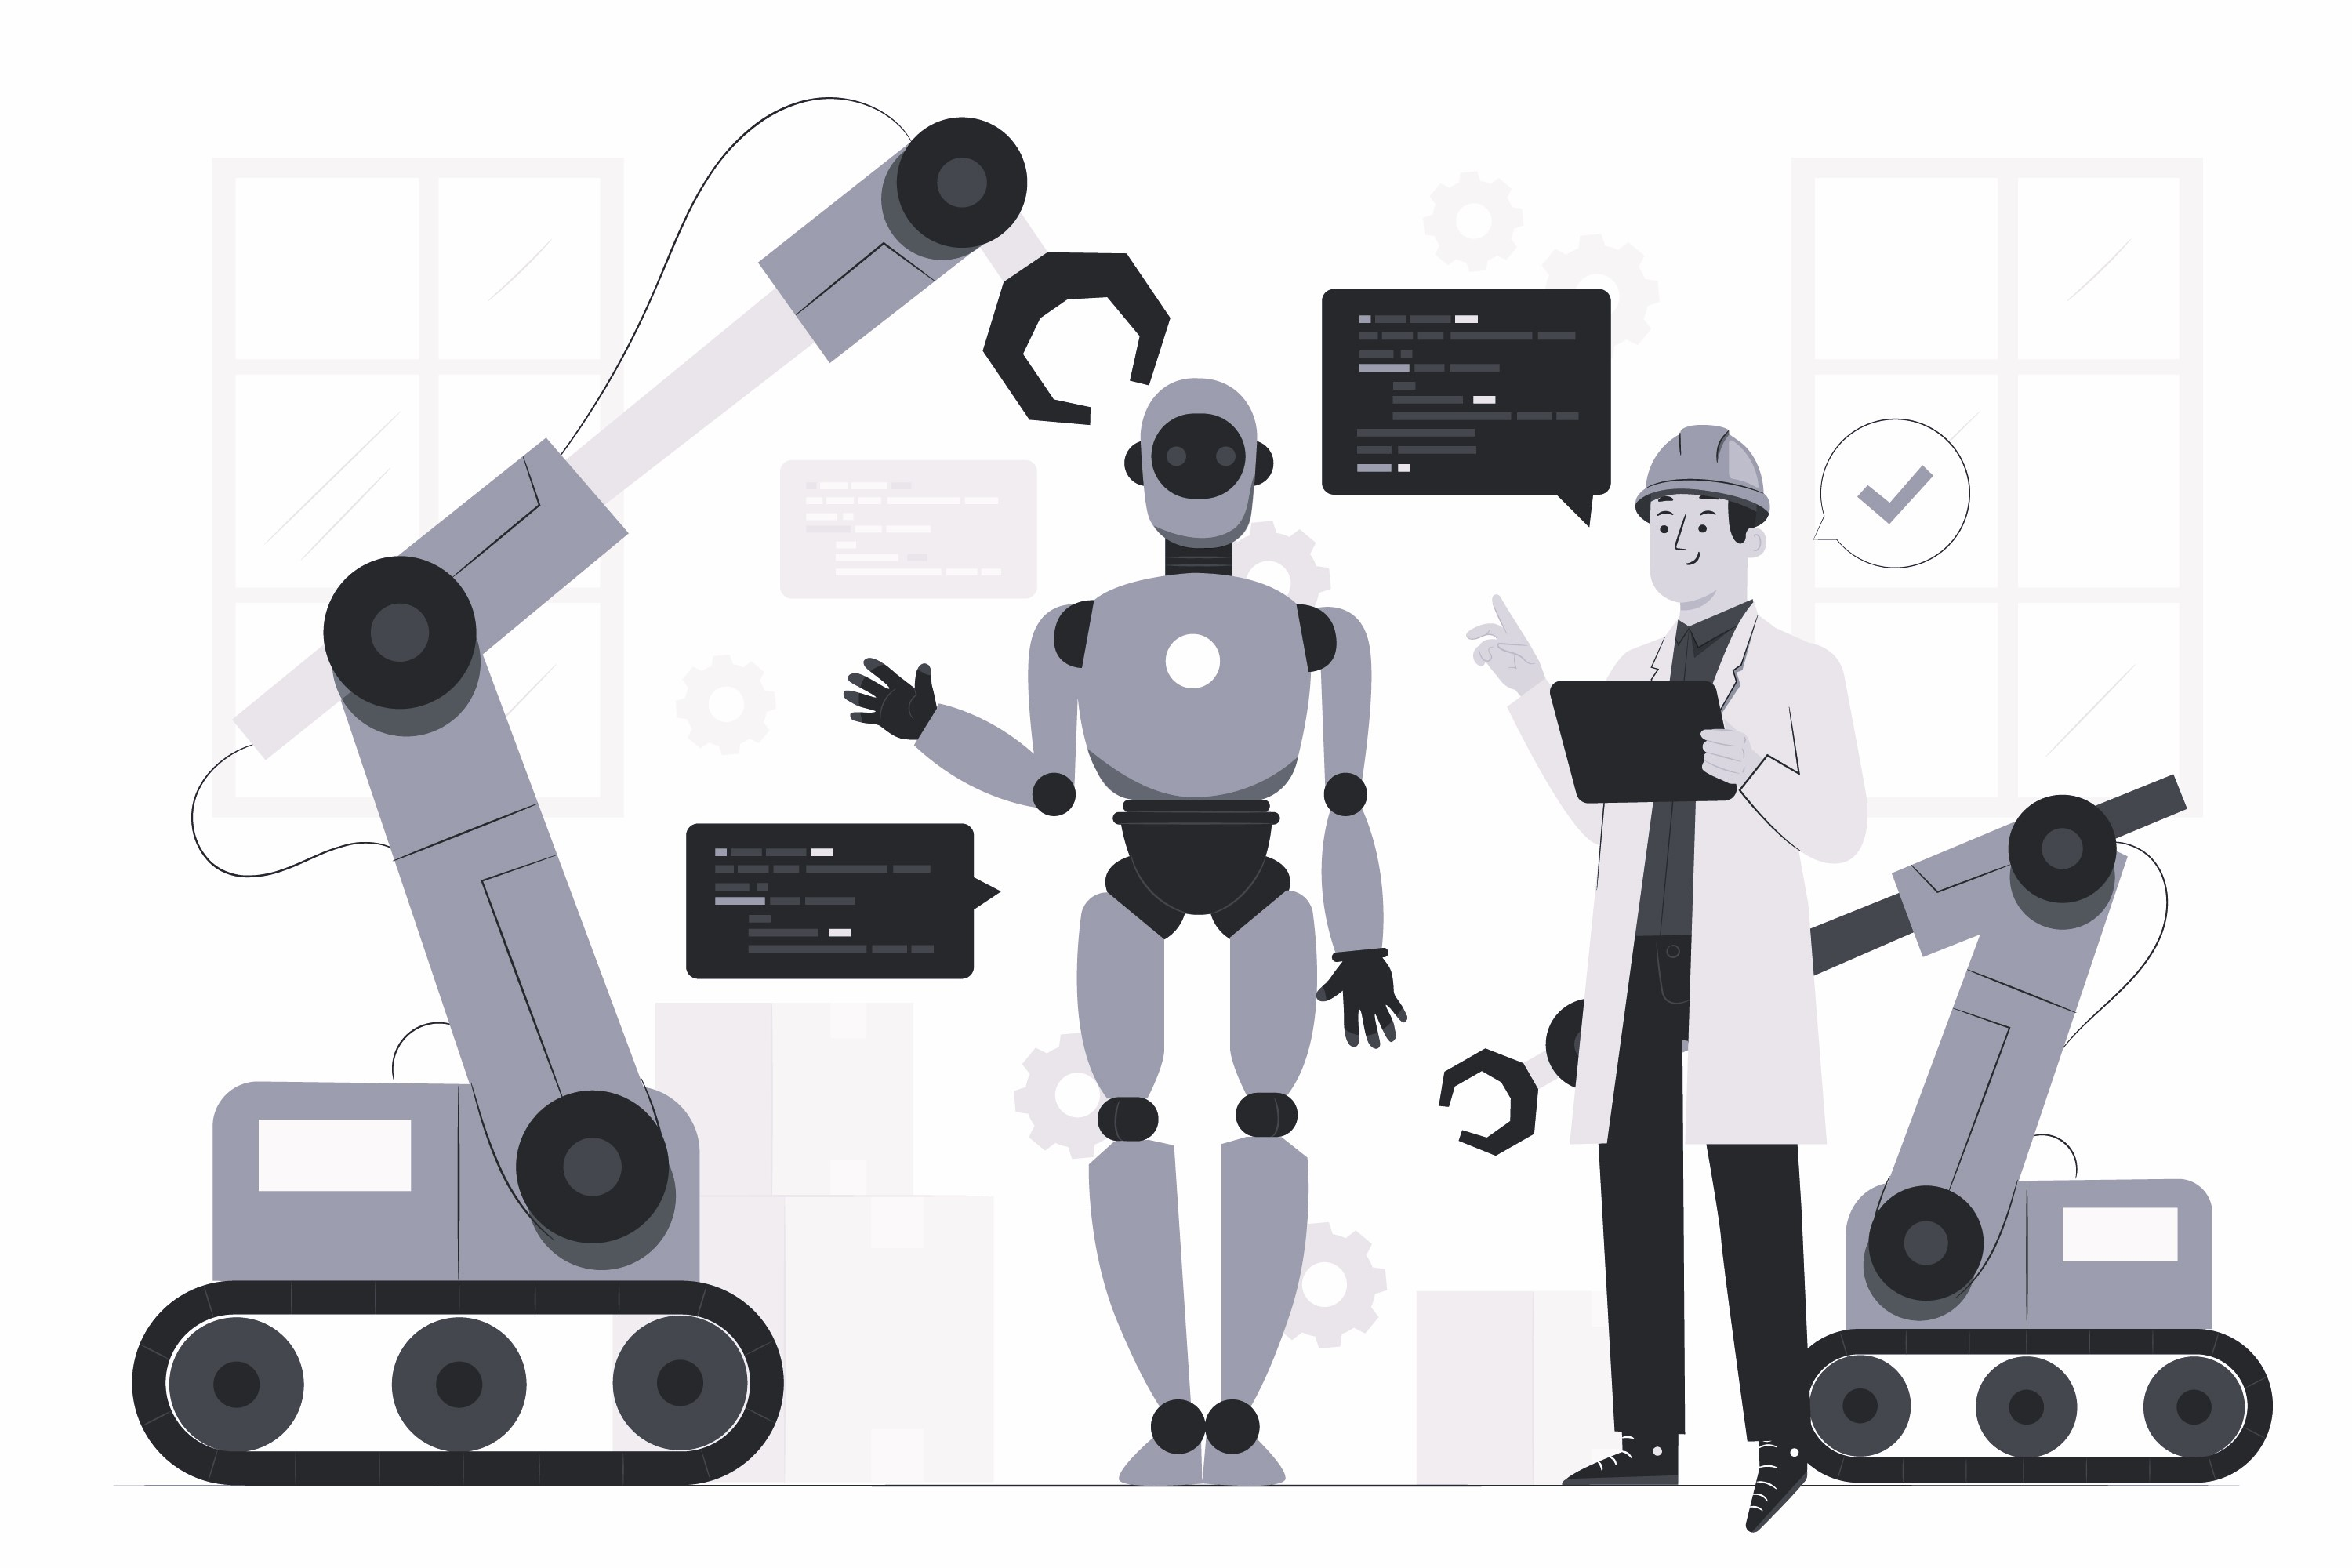
\includegraphics[scale=0.16]{img/8058233.jpg}\\[2cm]
    
    {\Large \textsf{Carlo Migliaccio}}\\[0.2cm]
    {\large \textsf{Master's Degree in Computer Engineering (LM-32)}}\\[1.5cm]
    {\large Academic Year 2024/25}\\[2cm]
    \vfill
\end{titlepage}
\newpage
\tableofcontents

\chapter{Introduction}
\begin{figure}[h]
    \centering
    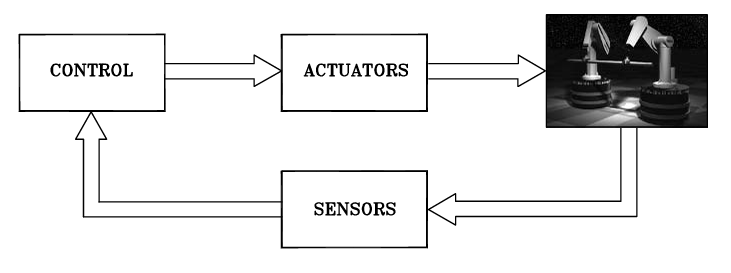
\includegraphics[scale=1]{img/robotic_system.png}
    \caption{Components of a robotic system}
\end{figure}
\vspace{-0.5cm}
\section{Robot: a possible definition}
\textit{What is robotics?} Before answering this question, it makes sense to rise up another question: \textbf{what is a robot?} Among all the available definitions the most suitable is the one provided by \textsf{Mike Brady}:
\begin{quotation}
    \colorbox{lightgray}{A robot realizes the \textit{intelligent} connection between \textbf{perception} and \textbf{action}.}
\end{quotation}
With reference to such a definition we can dissect it finding useful insights. A \textit{robotic system} is in the reality a complex system which is functionally represented by \textbf{multiple subsystems}. In particular you have a \textit{mechanical systems} which is made up of two apparatus: \textbf{locomotion apparatus} and a \textbf{manipulation apparatus} by which the robot itself can carry out the task. Both these subsystems are provided with an \textit{actuation system} which \textbf{animates} the mechanical part (this includes \textit{servomotors,drives} and \textit{transmissions})\footnote{
    It is quite clear that the \textbf{action} part is linked to the actuation system
}
The \textbf{perception} part rely on sensors which can acquire data about either the \underline{internal status} of the mechanical system (\textit{proprioceptive sensors}, eg. position transducers) or the \underline{external status} of the environments (they are called \textit{esteroceptive sensors}, eg. cameras).\\
The connection between the the actuation and sensing part is provided by a \textit{control system} which in an intelligent way can command the execution of some actions. It is remarkable that the control system exploits a mathematical model of the robot.\\
At this point, we can say that \textbf{Robotics} deals with
\begin{center}
    \Large
    \colorbox{lightgray}{\textbf{study} and \textbf{design} of robots.}
\end{center}
this is the reason why it results in an interdisciplinary subject involving \textit{mechanics, control, computers} and \textit{electronics}.\\
The term \textbf{robot} it is derived from the Slav term \textit{robota} (executive labor), and it appeared several years before any robot could be built!

\section{Robots classification}
Nowadays, robots can be used in different contexts according to which they are split in: 
\begin{itemize}
    \itemsep-0.2em
    \item \textsf{Industrial robots} they are used in the industrial field in order to perform several tasks such as soldering, moving part, cutting parts and so on; 
    \item \textsf{Humanoid and biometric robots} they are employed in order to interact with people or animal environments. Not rarely their mechanics is inspired by the real (natural) behaviour. 
    \item \textsf{Service robots} are used in contexts where the actions to be carried out are dangerous for human beings. For example: think about manipulating radioactive matter.
    \item \textsf{Exploration robots} are used, for example, in the field of space missions to study the atmosphere and the surface of Mars.
\end{itemize}

Another available classification of robots is the one based on the type of mechanical structure. Is the robot base moving or is it fixed? In the first case we are talking about \textbf{mobile robots} (humanoid/biometric, service and exploration robots often fall in this category), in the latter case we refer them with the term of \textbf{robot manipulators} (the great majority of industrial robots).

\subsection{Robot manipulator (Industrial robots)}
We anticipate here that a \textit{robot manipulator} is made up of a \underline{sequence of rigid bodies} (links) connected by means of articulations (\textit{joints}); the part of the manipulator that ensures mobility is the so-called \textbf{arm}, the part devoted to its agility (more technically, dexterity) is the \textbf{wrist} finally the part which perfors the action  is the \textbf{end-effector}. Several types of robot manipulators are obtained changing such components.

\begin{figure}
    \centering
    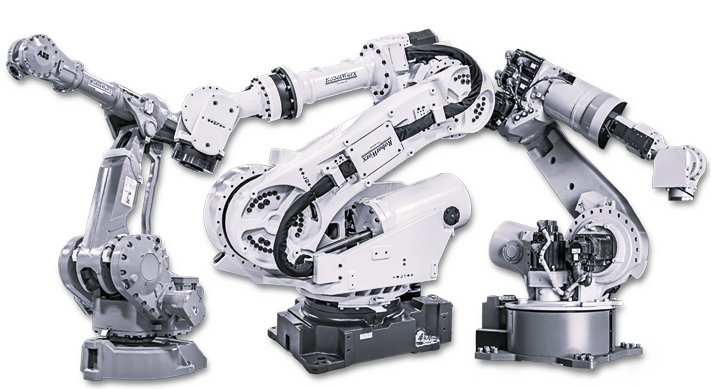
\includegraphics[scale=0.4]{img/3_Industrial_Robots.png}
    \caption{Examples of Industrial Robots}
\end{figure}

\subsection{Mobile robots}
The main feature here is the presence of a \textit{mobile base} which allows the robot to move into the environment it is placed. They are provided with a locomotion system that can be different (wheels, legs, wings...).



\section{Robot modeling, planning and control}
The totality of the tasks to be completed requires the execution of a \textit{specific motion prescribed to the robot}. The correct execution of the motion is entrusted to the control systems which should provide actuators with \textbf{command} consitstent with the desired motion (motion control), this -- in turn -- rely on an accurate analysis on the features of (jointly) mechanical structrure, actuators and sensors. The final aim of such an analysis is the derivation of a mathematical model describing the I/O relationship for the robot components (modeling component). Relevant topics in \textit{modeling, planning} and \textit{control} are briefly resumed in the following. 

\subsection{Modelling}
Obtaining a model for a robot (industrial or mobile) concerns essentially in studying both the \textbf{kinematics} and \textbf{dynamics}. The former is the description of the robot motion without taking into account forces and torques which causes it. The latter describes forces and torques which generates the motion.\\
A further distinction is made between between \textit{kinematics} and \textit{differential kinematics} is made. In the first case we want to find a relationship between the joints and end-effector positions. In the second case we want to study the relationship between the joint and end-effector motion by means of velocity. A very useful tool in this case is the \textit{Jacobian} of the manipulator.\\
We conclude this discussion by saying that having a model for the robot is useful for the mechanical design of the structure, choice of actuators, determination of control strategies and for doing computer-based simulations.

\subsection{Planning}
Every robot performs a task, for example for a manipulator we have the necessity to describe in some way the motion at the joints or at the end-effector. In material-handling task for example it is sufficient to decide an initial position and and end position (\textit{point-to-point} motion) in other situations we have to track a certain trajecotry (\textit{path motion}). In all these cases the task is the \textbf{trajectory planning} that is the determination of timing laws for relevant variables. For a mobile robot, such a task is even more complicate since it requires to take into account the constraints imposed by the wheels, legs, wings...

\subsection{Control}
The generated trajectories constitutes the reference signal for the \textit{control system} of the mechanical structure. Techniques for controlling manipulators and mobile robots are very different how we will see this is due the presence or not of the interaction robot-environment and of the mobile base.


%\chapter{Kinematics \colorbox{yellow}{\texttt{TO DO...}}}
\section{Rigid body pose}
\section{Rotation matrices}
\section{Composition of rotation matrices}
\section{Euler Angles}
\section{Angle-Axis representation}
\section{Quaternions}
\section{Homogeneous transformations}
\chapter{Mobile robots}
\vspace{-1cm}
\begin{figure}[h]
    \centering
    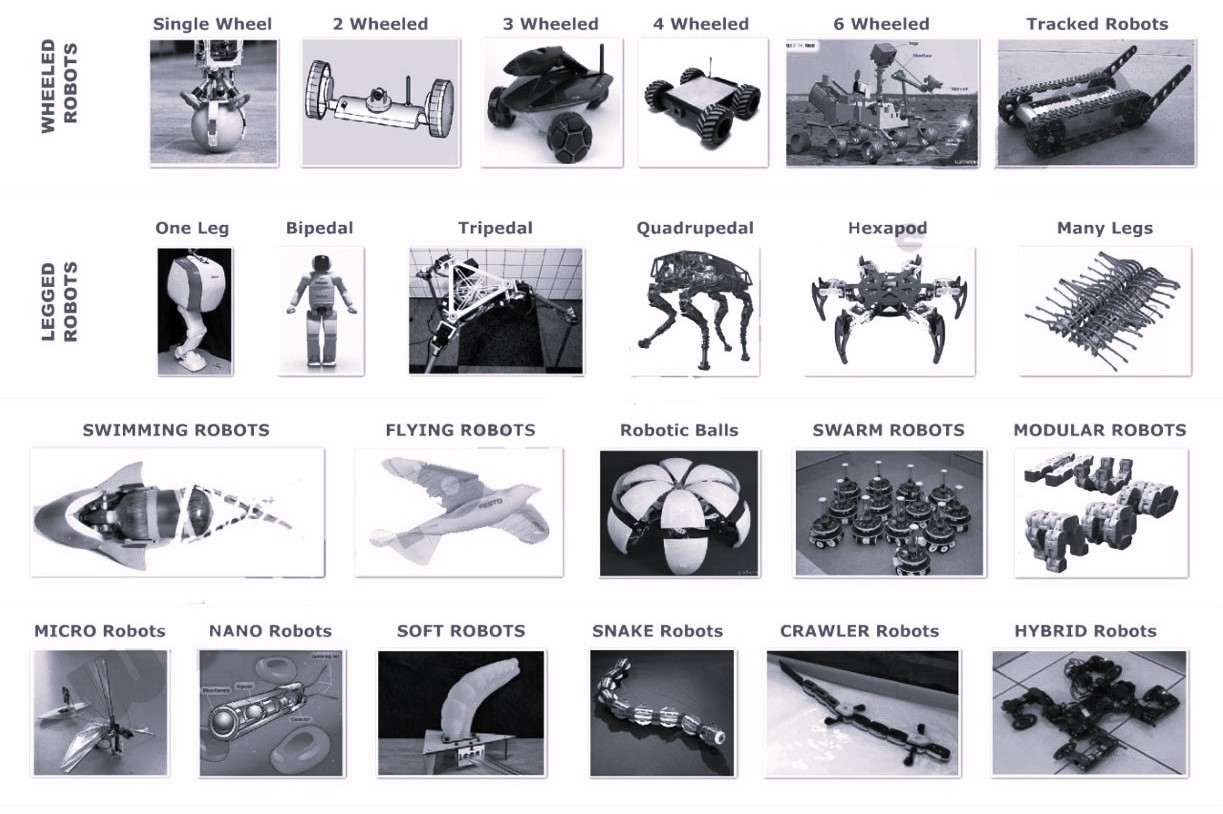
\includegraphics[scale=0.5]{img/classification.jpg}
\end{figure}
\vspace{-0.5cm}
\section{Introduction}
\begin{definition}[\textbf{Mobile robot}]
A \textbf{mobile robot} is a structure capable of moving and act in \textit{terrestrial}, \textit{underwater} or \textit{aerial} environments.    
\end{definition}
\noindent
The characteristics of the environment are fundamental since planning and control are affected by it. Namely the environment can be \underline{totally structured}, \underline{unstructured} or \underline{partially structured}. We refer the \textbf{structuredness} of the environment as the knowledge on geometric characteristics.
\subsection{Autonomy}
A mobile robot is equipped with a certain level of \textbf{autonomy} which makes the structure capable of moving independentlyh from a human supervisor. For achieving it, it is required a computational part (CPU, Intelligence of the robot), some sensors and actuators and an energy source, which can be either generated on-board or provided by mean of an external source.
\subsection{Locomotion}
Another fundamental aspect is that, differently from manipulators, a mobile robot is equipped with a \textbf{locomotion apparatus} which drastically changes according to the environment they are acting in. A \textbf{terrestrial robot} can have wheels, legs or a biomimetic locomotion system; a \textbf{underwater robot} can provided with propellers or water jets; finally, an \textbf{aerial robots} can have rotating, fixed or flapping wings.

\section{Types of wheels}
In the following we are focusing our attention on the wheeled robots, as they represent the great majority of mobile robots used in applications. The basic mechanical structure of this robot is indeed the wheel. The table \Cref{tab:wheels} shows a summary of the fundamental information about the most popular types of wheels.

\begin{table}
    \centering
    \begin{tabular}{m{5cm} m{9cm} m{2cm} }
        \textbf{WHEEL TYPE}&\textbf{DESCRIPTION}&\textbf{SYMBOL} \\
        \toprule
        {\textsc{Simple non-steering wheel}}&{They can rotate about an axis which passes  through the center of the wheel itself, orthogonal to its plane. The orientation of the chassis with respect to the wheels is constant.}&{\centering 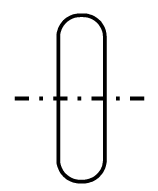
\includegraphics[scale=0.5]{img/simple_non_steering.png}} \\
        \midrule
        {\textsc{Simple steering wheels}}&{Has two axes of rotation, one that is orthogonal to the wheel plane, the other which is \textit{vertical} and goes through the center of the wheel. This provides the wheel with the possibility of changing the orientation with respect to the chassis. Note that for both non-steering and simple steering wheels the component the velocity which orthogonal to the wheel plane is null since there is no sleeping. That is: 
        \begin{equation*}
            v^{\perp}(t)=0
        \end{equation*}}&{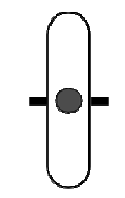
\includegraphics[scale=0.5]{img/simple_steering.png}} \\
        \midrule
        {\textsc{Castor wheel}}&{It is a variant of the previous one in which the vertical axis does not pass through the center of the wheel from which it is \textbf{displaced} by a constant offset. This adds degrees of freedom to the vehicle on which they are mounted on. Such a type of wheels are often used for office chairs and supermarket carts.}&{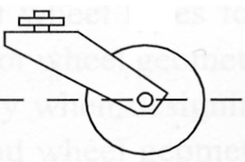
\includegraphics[scale=0.5]{img/castor_wheel.png}} \\
        \midrule
        {\textsc{Omnidirectional or Swedish wheel}}&{There is another type of non-conventional wheel that is the \textit{mechanum} (or \textbf{swedish wheel}). It mounts some passive rollers whose rotation axis is inclined by 45 degrees with respect to the plane of the wheel itself. They are also called \textit{omniwheels}.}&
        {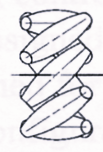
\includegraphics[scale=0.8]{img/swedish_wheel.png}} \\
        \midrule
        {\textsc{Spherical omniwheel}}&{There is another type of omniwheel which is \textbf{spherical}. They can be either active or passive. Like in the case of swedish wheels, a vehicle equipped with four of them is called \textbf{omnidirectional}.}& 
        {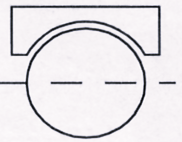
\includegraphics[scale=0.6]{img/spherical_wheel.png}}\\
    \end{tabular}
    \caption{Types of wheels with description and symbols}
    \label{tab:wheels}
\end{table}


\section{Constraints and Kinematic Models}
We have seen in the introduction that mobile and industrial robots have different characteristics, this results in different models, planning and control strategies. Since in general robots are made up of multiple rigid bodies (\textit{multibody system}) linked together by joints, their motion is constrained. This holds in general, however also the types of constraints are different in the case of mobile robots and manipulators. This is because in the former case you have limitations in the \textbf{position} of the whole body, in the case of mobile robots, and in particular in terrestrial wheeled robots, you have instead limitations on \textbf{how the position can change} in magnitude, direction and side (this is nothing but the \textbf{velocity}). From now on we are focusing our attention on \textbf{modeling wheeled robots}.

\subsection{Constraints and their classification}
In order to properly describing and giving a classification of constraints, it is better recalling the concept of \textbf{generalized coordinates}. \\
Let the vector $\mathbf{q}\in\mathbb{R}^n$ be the \emph{generalized coordinates} that describes the \textbf{configuration} of the robot (minimum number of variables needed to model the robot motion). For the moment, let us assume that the \textbf{configuration space} $\mathcal{C}$ coincides with $\mathbb{R}^n$. For example for a \textbf{unicycle} the generalized coordinates are in number of three: 
\begin{equation}\label{eq:gen_coord_unicyle}
    \mathbf{q}=[x \quad y \quad \theta]^T\in\mathbb{R}^3
\end{equation}
where $x$ and $y$ are the position of the contact point between the (single) wheel and the plane on which the motion occurs, while $\theta$ is the angle of the wheel with respect to the horizontal axis. The \textbf{evolution in time} of the generalized coordinates vector \textit{describe the motion} of the system.\\

Constraints can be found by mean of \textbf{equality} (in this case we refer them as \textit{bilateral} constraints), by mean of \textbf{inequality} (we refer them as \textit{unilateral} constraints). Furthermore, according to the fact they are or not time-variant, we can divide them in \textit{rehonomic} (explicit dependence on time) and \textit{scleronomic} (time-invariant constraints). In this course we will treat only \textbf{bilateral and scleronomic constraints} another term for indicating them is \textbf{holonomic} (or \textbf{integrable}) constraints.

\subsubsection{Holonomic constraints}
Such a type of constraint\footnote{
    We recall that for a multibody system described by using the Lagrangian approach, holonomic constraints are those allowing a reduction of the number of needed variables.
} can be expressed as: 

\begin{equation}
    h_i(\mathbf{q})=0, \quad i=1,...,k<n
\end{equation}

A system whose motion is characterized only by holonomic constraints is called \textbf{holonomic system}. By using the \textit{implicit function theorem} (or in Italian "Teorema del Dini"), we can reduce the dimension of the configuration space to $n-k$

\subsubsection{Kinematic constraints}
Such a type of constraints involve both generalized coordinates $\mathbf{q}$ and its derivative $\dot{\mathbf{q}}$. In the most general case they can be expressed as:
\begin{equation}
    a_i(\mathbf{q},\dot{\mathbf{q}})=0, \quad i=1,...,k<n   
\end{equation}
Kinematic constraints are limiting the set of generalized velocities that can be obtained by each configuration. In some cases they can be written in the so-called \textbf{Pfaffian form}, that is they can be written as a \textit{linear combination of the generalized velocities $\dot{\mathbf{q}}$}: 
\begin{equation}
    \mathbf{a}_i^T(\mathbf{q})\dot{{\mathbf{q}}}=0, \quad
    i=1,...,k<n
\end{equation}
An example of kinematic constraint in Pfaffian form is:
\begin{equation*}
    3q_1 \dot{q}_1 +
    2 \sin{q_1}\dot{q_2}+
    \sin{q_3} \dot{q}_3 =0   
\end{equation*}
The reason for using such a notation is that we can immediately retrieve the expression of the associated function by doing the row-by-column product (standard inner product). Such $k$ kinematic constraints can be written in compact form by introducing matrices
\begin{equation}\label{eq:matrix_pfaffian}
    \mathbf{A}^T(\mathbf{q})\dot{\mathbf{q}}=\mathbf{0}
\end{equation}
where $\mathbf{A(q)}\in\mathbb{R}^{k,n}.$ It is interesting to note that the presece of $k$ holonomic constraints imply the presence of $k$ kinematic constraints. This can be easily showed by computing the time derivative for the $k$ holonomic constraints: 
\begin{equation}\label{eq:kin_holonomic}
    \frac{d h_i(\mathbf{q})}{dt}=
    \frac{d h_i(\mathbf{q})}{d\mathbf{q}}\cdot
    \frac{d \mathbf{q}}{dt}=
    \frac{d h_i(\mathbf{q})}{d\mathbf{q}}\cdot \dot{\mathbf{q}}=0, \qquad
    i=1,...,k
\end{equation}
where we have applied the fact that the constraints are holonomic while using the \textit{Chain rule} for passing from the first to the second step. From the \Cref{eq:kin_holonomic} we have understood that: 
\begin{equation*}
    \text{holonomic constraint} \Longrightarrow 
    \text{kinematic constraints}
\end{equation*} 
In general, we cannot say the inverse and in this case (since the step from the derivative to the primitive results in doing the integral) associated constraints are called \textbf{nonholonomic} (or \textbf{non-integrable}) ones. A system characterized by such constraints is called \textbf{nonholonomic system}. In presence of non-integrable constraints the dimension of the configuration space $\mathcal{C}$ cannot be reduced while the generalized velocities can be described over a subspace of dimension $n-k$ (how we are going to see in a minute).

\subsubsection{Example of nonholonomic constraint}
A unicycle rolls on a plane \textbf{without slippering}, we have already seen its generalized coordinates. For such a system we have the so called \textbf{pure rolling constraint}, this imply the velocity of the contact point not to have a non-zero component along the direction orthogonal to the wheels plane. By using simple trigonometric properties involving the inifinitesimal increment $dx$ and $dy$, we can state that
\begin{equation}
    \frac{dy}{dx}=\tan{\theta}
\end{equation}
Can we obtain the Pfaffian form for such a constraint? The answer is YES. In fact by dividing and multiplying for an infinitesimal time increment $dt$ we obtain:
\begin{equation*}
    \frac{dy}{dx}=\frac{dy}{dt}\cdot
    \frac{dt}{dx}=\frac{\dot{y}}{\dot{x}}=\frac{\sin\theta}{\cos{\theta}} \iff 
    \dot{y}\cos{\theta}=\dot{x}\sin{\theta}
\end{equation*}
Which is the same to say that
\begin{equation}
    \dot{x}\sin\theta-\dot{y}\cos{\theta}=0 \iff 
    [\sin\theta \quad \cos\theta \quad 0] \dot{\mathbf{q}}=0
\end{equation}
The constraint we have just derived can be demonstrated that is non-integrable and so nonholonomic, in fact we cannot reduce the dimension of the configuration space (in other words all of the generalized coordinates are needed to properly describe the unicycle motion). Note that, start from an initial state $\mathbf{q}_i$, you can bring the system to any final state $\mathbf{q}_f$, under the assumption of not to violating the pure rolling constraint\footnote{
    We will see that in order to pass from an initial to a final state a \textit{trajectory planning algorithm} must be used.
}.

\subsection{Kinematic model}
From the \Cref{eq:matrix_pfaffian}, we can immediately see that the $n-k$ admissible generalized velocities belong to the null space\footnote{
    Just for doing a brief recap. Given a matrix $A\in\mathbb{R}^{m,n}$ we can individuate the following sets (vector spaces):
    \begin{itemize}
        \itemsep-0.3em
        \item \textsf{Null space} that is the a subset of $\mathbb{R}^n$ defined as: 
        \begin{equation}
            \mathcal{N}(A)=\{x\in\mathbb{R}^n: \ Ax=0\}
        \end{equation}
        \item \textsf{Range space} that is a subset of $\mathbb{R}^m$ defined as: 
        \begin{equation}
            \mathcal{R}(A)=\{y\in\mathbb{R}^m: \ y=Ax\}
        \end{equation}
        the dimension of such a vector space is called the rank of the matrix A (rank(A)) and it holds that its maximum value is the $\min(m,n)$.
    \end{itemize}
    Another important result is that
    \begin{equation*}
        n=\dim{\mathcal{N}(A)}+\dim{\mathcal{R}}(A)
    \end{equation*}
    Knowing $n$ (for us dimension of the configuration space)
 and the rank of A, we can find the dimension for the null space of A.} of $\mathbf{A(q)}^T$ that is 
\begin{equation}
    \dot{\mathbf{q}} \in \mathcal{N}(\mathbf{A^T(q)})
\end{equation}
We know that this is a vector space and it has got a basis of $n-k$ elements which we can denote with $\{\mathbf{g}_i(\mathbf{q})\}_{i=1}^{n-k}$, we can group together such elements in a matrix $\mathbf{G(q)}$ so that the generalized velocities can be expressed as
\begin{equation}
    \mathbf{\dot{q}=G(q)u}
\end{equation}
this is nothing but the \textbf{kinematic model} of the constrained system. The vector $\mathbf{q}$ is called the \emph{state vector} while $\mathbf{u}$ is the \textbf{input vector}. Moreover the obtained system is said to be driftless since in absence of an input the generalized velocity is null. Not rarely the components $u_i$ of \textbf{u} have a meaning related to the physics or the available control input.\\

In the following for better fixing the concepts we have just given, two example of kinematic models are given.

\subsubsection{Kinematic model for the unicycle}
Let us consider, a bit more in details, the unicycle system. It is noticeable that the line in which the motion does not occur is called \textbf{zero motion line}.\\
We have said that the generalized coordinated $\mathbf{q}$ are the ones in \Cref{eq:gen_coord_unicyle}. We have a single constraint that we have reduced in Pfaffian form. The next step \emph{in order to obtain a kinematic model} is determining a base for the null space of the constraint matrix. One possible choice for vector fields $\mathbf{g_i(q)}$ is\footnote{
    Note that this is a vector field since both domain and codomain are vectors of suitable dimensions.
}:
\begin{equation*}
    \mathbf{g}_1(\mathbf{q})=\begin{bmatrix}
        \cos\theta&\sin\theta&0
    \end{bmatrix}^T, \quad
    \mathbf{g}_2(\mathbf{q})=\begin{bmatrix}
        0&0&1
    \end{bmatrix}^T
\end{equation*}
\begin{multicols}{2}
    \noindent
    Therefore, putting them together we obtain the matrix
\begin{equation}
    \mathbf{G(q)}=\begin{bmatrix}
        \cos\theta&0\\
        \sin\theta&0\\
        0&1
    \end{bmatrix}
\end{equation}
The kinematic model for the unicyle, then, can be written as:
\begin{equation}
    \begin{bmatrix}
        \dot{x}\\\dot{y}\\\dot{\theta}
    \end{bmatrix}=\begin{bmatrix}
        \cos\theta\\
        \sin\theta\\
        0
    \end{bmatrix}v+\begin{bmatrix}
        0\\0\\1
    \end{bmatrix}\omega
\end{equation}
\\
\begin{figure}[H]
    \centering
    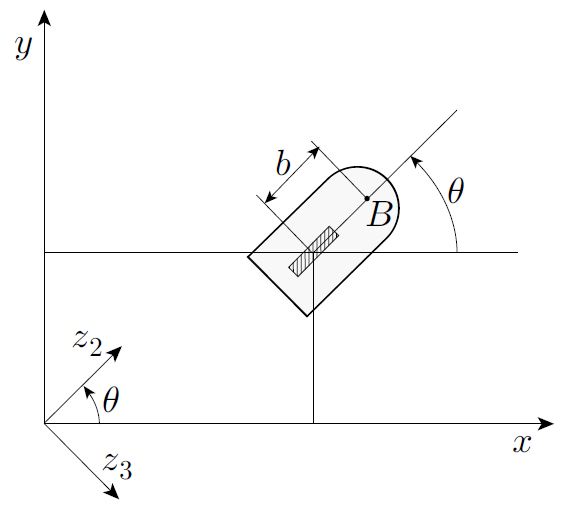
\includegraphics[scale=0.6]{img/unicycle_scheme.png}
    \caption{Choice of generalized coordinates for the unicycle}
    \label{fig:unicycle_model}
\end{figure}
\end{multicols}
In such a context the elements of the input vector have a physical meaning, since $v$ is the driving velocity, while $\omega$ is nothing but the steering velocity.  Why are we interested in studying the kinematic model of a unicyle? Consider that without a human beings balancing the system this is also an unstable system! However, there are some robot (stable) robot structures that from a \textbf{kinematic point of view} are equivalent to unicycles. We are talking about \emph{differential drive} and \emph{synchro drive} vehicles.

\subsubsection{Kinematic model for a bicycle}
A \textbf{bicycle} is vehicle with a steered wheel and a fixed one, the distance between the wheels is fixed to be $L$. As usual we have to choose the (generalized) coordinates for such a vehicle a possible choice is the following:
\begin{itemize}
    \itemsep-0.3em
    \item $(x,y)$ being the contact point of the rear\footnote{
        back wheel
    }; 
    \item $\theta$ is the angle between the rear wheel and the $x$ axis (this is nothing but the orientation of the vehicle with respect to the $x$ axis); 
    \item $\phi$ is the steering angle of the front wheel.
\end{itemize}
\begin{remark}
    It is interesting focus our attention on a point: why do not we introduce also the coordinates of the front wheel? Well, it is sufficient having a single contact point since, back and front wheel are at a fixed distance $\ell$, and this is nothing but an \textit{holonomic constraint} which allows us the shrinking of the configuration space dimension! 
\end{remark}
Going on into the discussion, there are essentially two \textit{pure rolling constraints}, one for each wheel: 
\begin{align}
    &\dot{x}_f \sin(\theta+\phi)-\dot{y}_f \cos(\theta+\phi)=0 \label{eq:front_pure_rolling}\\
    &\dot{x}\sin(\theta)-\dot{y}\cos(\theta)=0
\end{align}
while indicating with $(x_f,y_f)$ the coordinates of the front wheel center, while $(\theta+\phi)$ is its angle with respect to the fixed reference frame. We have just said that they are not strictly necessary, since they can be obtained starting from the coordinates of the other wheel in particular: 
\begin{equation}
    \begin{cases}
        x_f=x+\ell\cos\theta\\
        y_f=y+\ell\sin\theta
    \end{cases}
\end{equation} 
using the trigonometry, the \Cref{eq:front_pure_rolling} can be expressed as
\begin{equation}
    \dot{x}\sin(\theta+\phi)-\dot{y}\cos(\theta+\phi)-\ell\dot{\theta}\cos(\phi)=0
\end{equation}
where we have used that $\sin^2\theta+\cos^2\theta=1$ and the trigonometric formulas for $\cos(\theta+\phi)$ and $\sin(\theta+\phi)$. The derived constraints can be put if Pfaffian form using the matrix
\begin{equation}
    \mathbf{A}^T(\mathbf{q})=\begin{bmatrix}
        \sin\theta&-\cos\theta&0&0\\
        \sin(\theta+\phi)&-cos(\theta+\phi)&-\ell\cos\phi&0
    \end{bmatrix}
\end{equation}
\begin{multicols}{2}
    
\noindent 
Our objective is obtaining a basis for the null space of such a matrix in order to derive the kinematic model. Since $rank(\mathbf{A^T(q)})=2$, the dimension of its null space is given by the difference between the dimension of the configuration space and such a rank, that is 2. A possible basis for such a null space is given by the column of
\begin{equation}
    \mathbf{G(q)}=\begin{bmatrix}
        \cos\theta\cos\phi&0\\
        \sin\theta\cos\phi&0\\
        \frac{\sin\theta}{\ell}&0\\
        0&1
    \end{bmatrix}
\end{equation}
\begin{figure}[H]
    \centering
    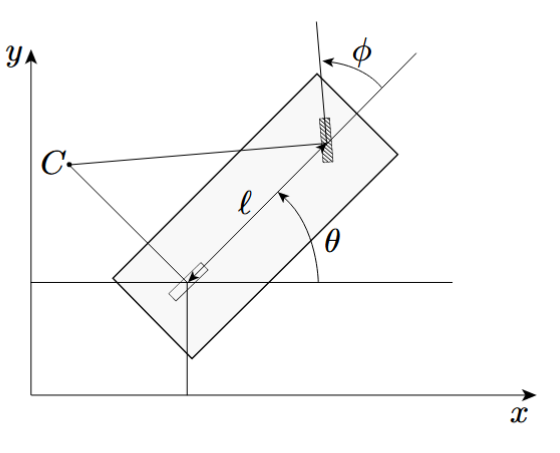
\includegraphics[scale=0.6]{img/bicycle_scheme.png}
    \caption{Possible choice for the generalized coordinates of a unicycle}    
    \label{fig:scheme_bicycle}
\end{figure}
\end{multicols}
\noindent
The associated kinematic model is:
\begin{equation}
    \begin{bmatrix}
        \dot{x}\\
        \dot{y}\\
        \dot{\theta}\\
        \dot{\phi}
    \end{bmatrix}=\begin{bmatrix}
        \cos\theta\cos\phi\\
        \sin\theta\cos\phi\\
        \frac{\sin\theta}{\ell}\\
        0
    \end{bmatrix}u_1 + \begin{bmatrix}
        0\\
        0\\
        0\\1
    \end{bmatrix}\omega
\end{equation}
the control input $u_1$ can be choosen according to the drive in particular $u_1=v$ if the vehicle is front-drive, $u_1=v/\cos\theta$ if the vehicle is back drive, since the first two equations must be equivalent to the ones of a unicyle. Just for a matter of notation/nomenclature the instersection point $C$ between the two zero motion lines is called \textit{instantaneous center of rotation}, depends only on $\mathbf{q}$ and it is interesting since each point of the chassis is moving instantaneously along along the circumference centered at $C$ (see \Cref{fig:scheme_bicycle}).\\
Equivalent (stable) systems having the same kinematic model are the \textbf{tricyle} and the \textbf{automobile}.

\section{Sensors for mobile robots}


\chapter{Kinematics of manipulators}
\begin{quotation}
    \noindent\textsf{
        In this chapter we will talk about \textit{kinematics of manipulators}. How we will see, they are totally different with respect to mobile robots: if for mobile robots we have a moving chassis mounted on wheels, on the other hand we have chains of links and joints. This is due to substancial mechanical difference among the two cateogories. We will give an introduction on the structure of such robots (joint, links, wrists...) and then we will describe the \textit{direct kinematics problem} and the \textit{inverse kinematics problem}.
    }
\end{quotation}
\minitoc

\section{Kinematic chains}
The \textbf{Kinematics} allows us to study the \textit{position, velocity and acceleration} of particular points of a multibody system independently from forces and torques that generated them. In order to describe the \textit{kinematic for manipulator} the definition of \textbf{kinematic chain} is needed.
\begin{definition}[Kinematic chain]
    A \textbf{kinematic chain (KC)} is a series of ideal arms/links connected by ideal joints.
\end{definition}
For our purposes a KC is only a geometric entity, we will not consider mass, inertia, friction and so on. More specifically:
\begin{itemize}
    \itemsep-0.3em
    \item \textit{links/arms} are idealized with geometric bars connecting two or more joints; 
    \item \textit{Joints} are idealized physical components allowing a relative motion among consecutive arms. Each joint provides a \textbf{degree of motion}.
\end{itemize}

\begin{figure}
    \centering
    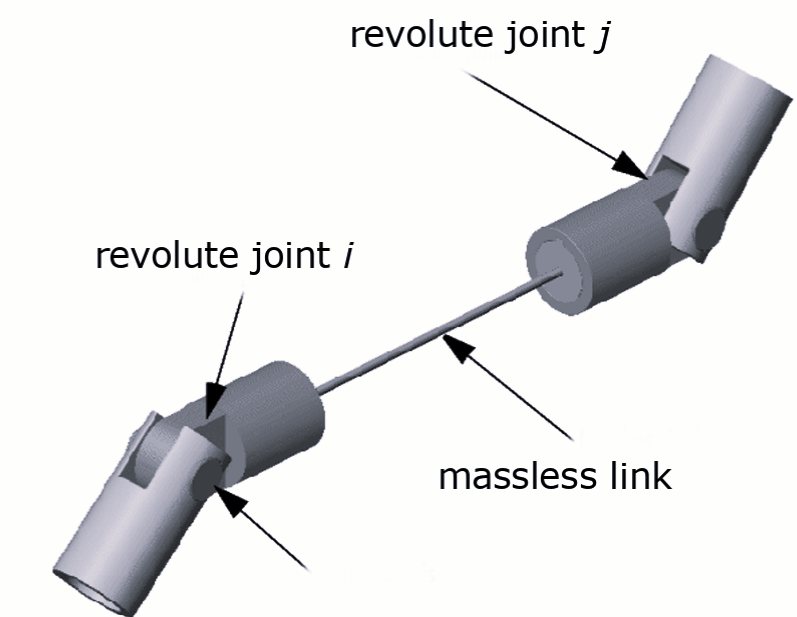
\includegraphics[scale=0.5]{img/joints_links.png}
    \caption{The robot joints are moved by actuators (eg. motors) and are connected by links/arm which are assumed to be massless}.
\end{figure}
\newpage
\subsection{Types of joints}
In the following we will consider two types of joints: 
\begin{enumerate}
    \itemsep-0.3em
    \item \textsf{Revolute (or Rotational) joints} which allows a \textbf{rotation} between the connected links; 
    \item \textsf{Prismatic (or Traslational) joints} which allows a \textbf{translation} between the connected links.
\end{enumerate}

\begin{figure}
    \centering
    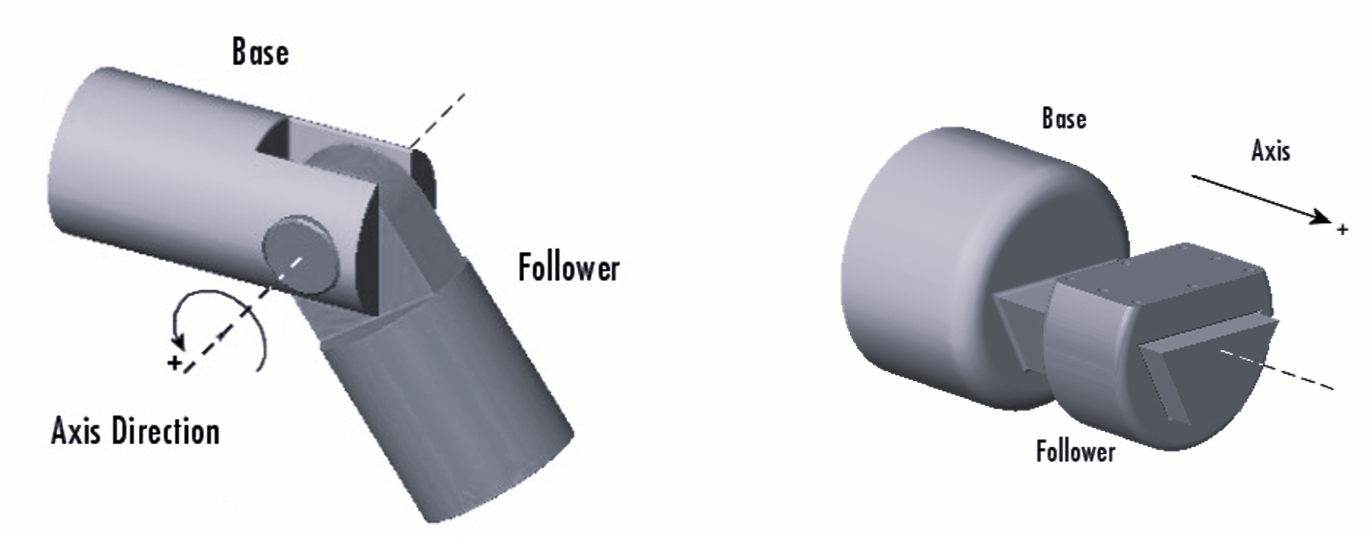
\includegraphics[scale=0.5]{img/joints_tyeps.png}
    \caption{Revolute and Prismatic joints. With a dashed line the direction of motion (axis) is indicated}
\end{figure}
According to the number of links we can find between any two joints, kinematic chains can be \textbf{open chains} or \textbf{closed chains}. In the former case there is only one link between any two links in a way joints and arms form a \textit{tree-like} structure; in the latter case there might be more than one link between any two joints, and in this case joints and arms are arranged in a \textit{cycle-like} structure.

\subsection{Graphical representation}
There are different types of graphical representations for kinematic chains, in the following we will use cylinders and boxes for joints, segment for links/arms. 

\begin{figure}
    \centering
    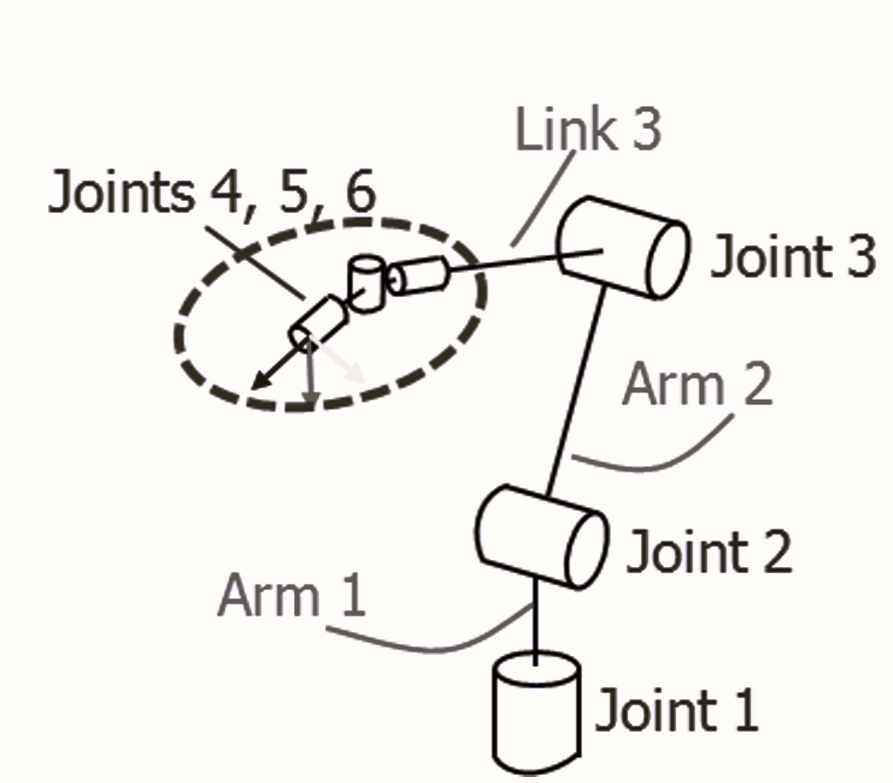
\includegraphics[scale=0.5]{img/KC_sample.png}
    \caption{Kinematic chain sample}
    \label{fig:KC_sample}
\end{figure}
More specifically \textit{\textbf{rotation joints}} are drawn in 3D has small cylinders withb the axes aligned along each rotation axis, in 2D they are drawn as small circles or small hourglasses.

\begin{figure}[h]
    \centering
    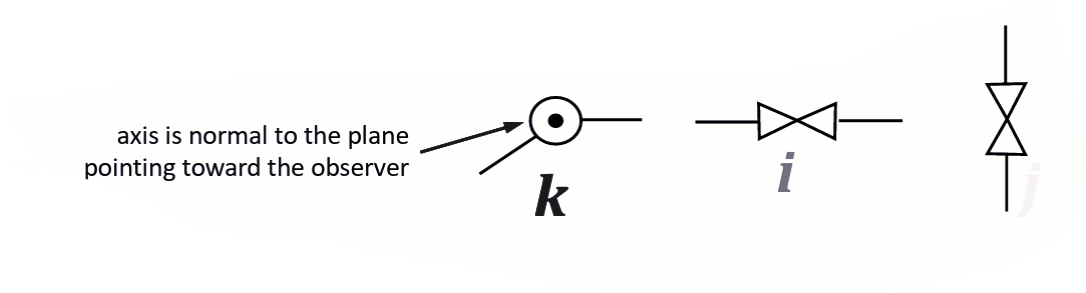
\includegraphics[scale=0.6]{img/rot_joints.png}
    \caption{2D-representation for revolute joints}
\end{figure}

At the opposite, \textit{\textbf{prismatic joints}} are represented as small boex with each axis aligned along the translation axis. On the other hand in 2D they are drawn as small squares with a point in their center, or as small rectangles showing the direction for the outcoming links.

\begin{figure}
    \centering
    
\includegraphics[scale=0.5]{img/transl_joints.png}
    \caption{2D representation of translational joints}
\end{figure}

\begin{figure}
    \centering
    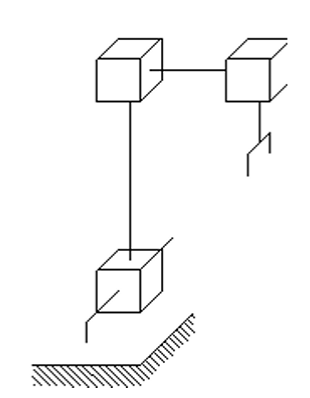
\includegraphics[scale=0.6]{img/transl_joints_3D.png}
    \caption{3D graphical representation for prismatic joints}
\end{figure}

\subsection{End-effector}
The \textbf{end-effector} (also called \textit{hand, gripper} or \textit{hand tool}) is the structure which is attached to the last link, and it is the one by which the task, for which that robot was introduced, can be executed. For the end effector a particular type of point is interesting, this is the \textbf{Tool Center Point (TCP)} and it is the baricenter of the hand, or better that ideal point that the robot software moves through the space. How we will see it is useful to attach to such a point a reference frame. \\
The graphical representation is used for the end-effector is a sort of fork. The end-effector can be of any type and we can draw and study the kineamtic chain without assuming the use of any particular hand.

\begin{figure}
    \centering
    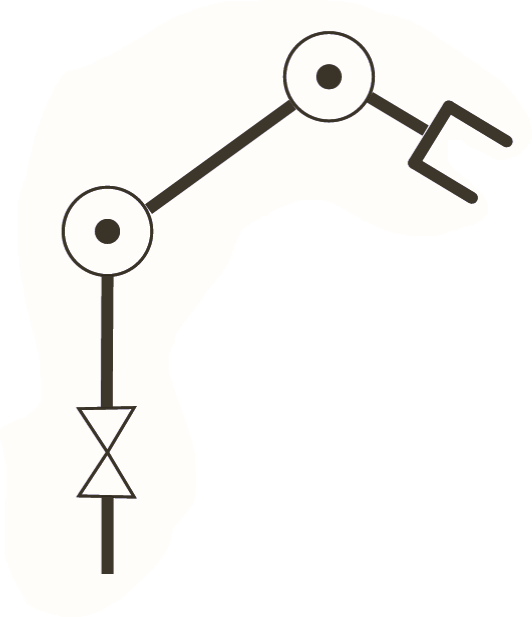
\includegraphics[scale=0.4]{img/endeff_graphical.png}
    \caption{End-effector graphical representation. Typically the TCP is assumed to be the center of the 'fork'}
\end{figure}




\section{Robot types}
An \textbf{Industrial manipulator} is usually composed by a \textbf{shoulder} and a \textbf{wrist}. The manipulators can be categorized according to the structure of their arms, which are based on the type of joints. We will indicate:
\begin{center}
    \underline{\textbf{R=revolute joint}}\\
    \underline{\textbf{P=Prismatic joint}}
\end{center}
A great number of robots can be obtain according the shoulder configuration, however in the industrial fields, few configurations are used which are more suitable for certain tasks instead of others. In the following \Cref{tab:manip_types} we are going to explore the most common structures giving their main characteristics.

\begin{longtable}{c c m{8cm}}
    \caption{Common types of manipulators}\\
    \hline
    \textbf{Robot type} & \textbf{Image} & \textbf{Description} \\
    \hline
    \endfirsthead

    \hline
    \textbf{Robot type} & \textbf{Image} & \textbf{Description} \\
    \hline
    \endhead

    \hline
    \endfoot

    \hline
    \endlastfoot\\
    \caption{Common types of manipulators}\label{tab:manip_types}\\

    \textbf{Cartesian Manipulator} & 
    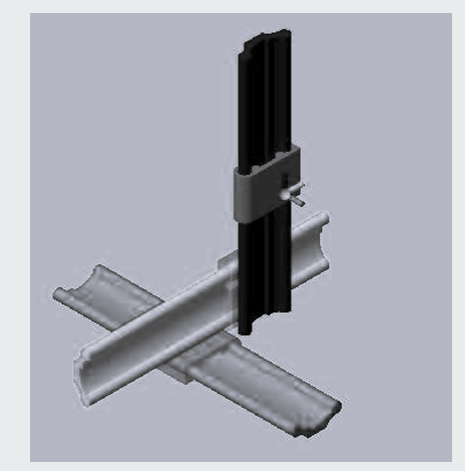
\includegraphics[width=3cm]{img/man_cart.png} & 
    In a \textbf{cartesian manipulator} the structure \texttt{(PPP)} is related to the shoulder structure. In this case the shoulder is composed of three prismatic joints, whose axis are mutually orthogonal. In this case, each degree of motion corresponds to a cartesian variable. We anticipate that the task space is a sort of \textit{parallelepiped}. Such robots have good accuracy, while regarding dexterity, it cannot be said the same. \\
    \hline
    \textbf{Cylindrical Manipulator} & 
    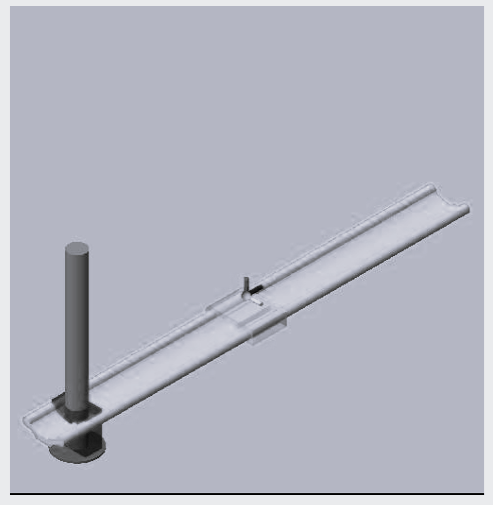
\includegraphics[width=3cm]{img/cyl_man.png} & 
    One rotoidal joint and two prismatic joints are the basic building blocks for the shoulder of a cylindrical manipulator. Each DOM (degree of motion) corresponds to a cylindrical coordinate. The \textit{task space} is a \textbf{cylindrical sector}. The horizontal prismatic joint allows reaching horizontal spaces; however, the accuracy decreases toward the arm ends. \\
\hline
    \textbf{Spherical Manipulator} & 
    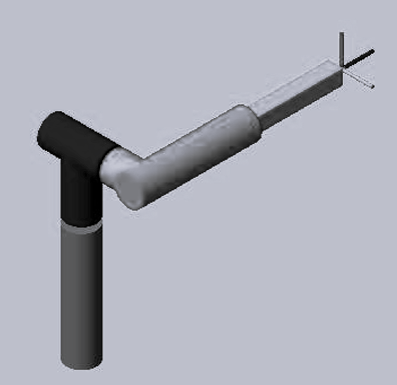
\includegraphics[width=3cm]{img/spherical_man.png} & 
    For a \textbf{polar (or spherical) manipulator}, the shoulder has two revolute joints followed by a prismatic one. Each DOM corresponds to a polar coordinate; here, the task is a spherical sector that may include parts of the floor to allow the manipulation of objects there located. The structure is less rigid compared to previous ones, and the accuracy reduces with the elongation of the prismatic arm. \\
\hline
    \textbf{SCARA \texttt{(RRP)}} & 
    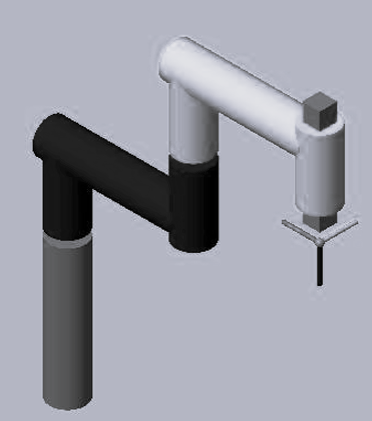
\includegraphics[width=3cm]{img/scara.png} & 
    It is a robot used for \textit{pick and place} applications. The shoulder has two revolute joints followed by one prismatic joint, all with \textbf{parallel vertical axes}. The tasks addressed by this robot are the manipulation of small components or little assembly tasks. \\
\hline
    \textbf{Antropomorphic} & 
    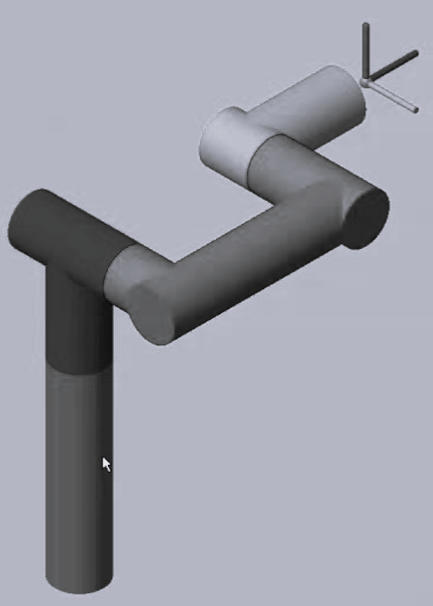
\includegraphics[width=3cm]{img/antrop_man.png} & 
    The shoulder is composed of \textbf{three revolute joints}: the first one is vertical, the others are \textbf{horizontal and parallel}. It is one of the most common structures in the industry since it is the robot having \textbf{the best dexterity}. \\
\hline
    \textbf{Parallel robots}&{
        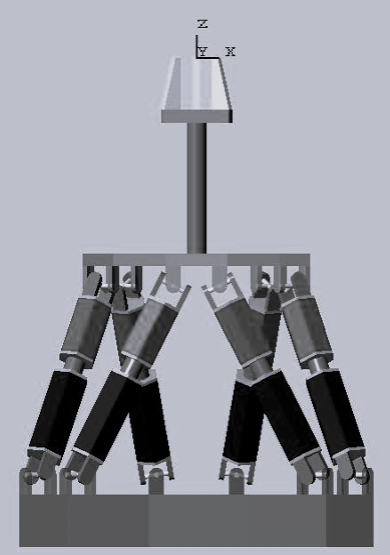
\includegraphics[width=3cm]{img/parallel_man.png}
    }&{
        Such a type of manipulators have joints and links forming a cycle-like structure. They are not covered in these notes. An example is showed in the figure aside.
    }\\
    
\end{longtable}
%------------------------------------------------------------


\section{Wrists}
The main scope of the \textbf{wrist} is to \textit{give an orientation} to the TCP. In fact, it can be said that the shoulder sets the \textbf{origin position}, while the \textbf{wrist} orients the TCP. \textit{Spherical wrists} are the most common. A wrist is said to be \textbf{spherical} if the three axes always intersect in a single point.Even if not spherical, due to its orientation function, the wrist is made up of \textbf{three rotational joints}.

\begin{figure}[h]
    \centering
    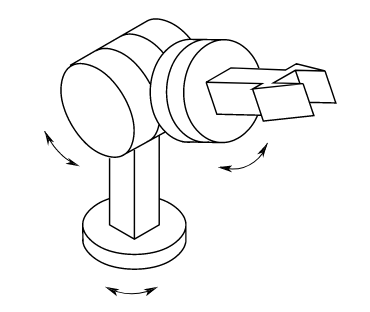
\includegraphics[scale=0.7]{img/polso.png}
    \caption{Spherical wrist}
\end{figure}
Taking into account a spherical joint, simplifies a lot the tractation of related topics of both manipulator kinematics and dynamics. Looking at the \Cref{fig:KC_sample} the wrist is the terminal part made up of joints 4,5,6.
 
\section{Direct Kinematics}
Many times in robotics there is the need to connect the "external world" to "robot world". In studying the kinematics of a manipulator the questions can arise are:
\begin{enumerate}
    \item Where is the end-effector given the information about the joints? (This is known as the \textbf{Direct kinematics problem}).
    \item What is the position of the joints to have in order to obtain a certain position of the end-effector? (This is known as the \textbf{Inverse kinematics problem})
\end{enumerate}
More specifically, the information about the joints are given by using \textbf{joint variables}, how we will see in explaining the Denavit-Hartemberg convention.

\begin{comment}
\begin{figure}[h]
    \centering
    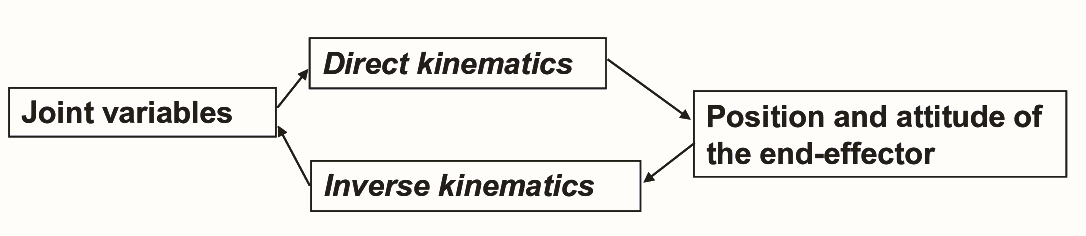
\includegraphics[scale=0.6]{img/direct_inverse_kinematics.png}
\end{figure}
\end{comment}

\begin{figure} [h]
    \centering
    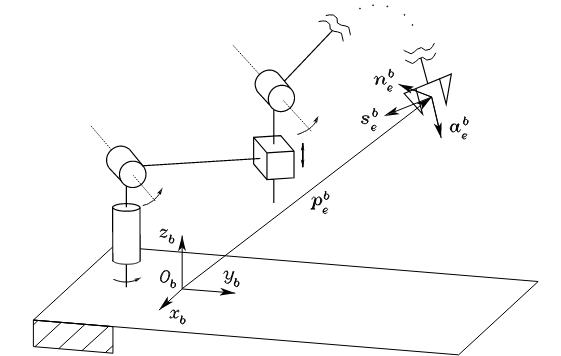
\includegraphics[scale=0.8]{img/kinematic_chain.png}
    \caption{Kinematic chain: joints and arms}
    \label{fig:chain}
\end{figure}
From now on, we are considering a manipulator consisting of $n+1$ links conected in an open chain through the use of $n$ joints\footnote{It is sufficient to think that for a joint is for two links.}.\\
With respect to the reference frame attached to the base of the robot $\mathcal{R}_b=\{O,x_b,y_b,z_b\}$ the \textbf{direct kinematic function} is expressed in term of the homogeneuous transformation matrix 
\begin{equation}
    \bb{T}_e^b(\bb{q})=\begin{bmatrix}
        \bb{n}_e^b(\bb{q})& \bb{s}_e^b(\bb{q})& \bb{a}_e^b(\bb{q})& \bb{p}_e^b(\bb{q})\\
        0&0&0&1
    \end{bmatrix}
    \label{eq:homtransform}
\end{equation}
where $\bb{q}$ is the vector containing the \textbf{joint variables} for the $n$ joints. While $\mathcal{R}_e=\{O_e,n_e,s_e,a_e\}$ is a reference frame related to the end-effect (this is chosen according to the specific task geometry). 
Some further clarification about $\mathcal{R}_e$. If the end-effector is a gripper the origin of the frame is put in the TCP, the unit vectors are: 
\begin{enumerate}
    \itemsep-0.3em
    \item $\bb{a}$ stands for \textbf{approach}, lays along the approach direction; 
    \item $\bb{s}$ stands for \textbf{sliding} lays along the sliding plane of the gripper jaws.
    \item $\bb{n}$ completes the right-handed frame.
\end{enumerate}
A first approach to use to obtain the \Cref{eq:homtransform} is by inspection  and using geometrical considerations. A more efficient and relatively \textit{effortless approach} is to use a systematic procedure. Things are made even more complicate when there are two or more closed kinematic chains. In the following we are going to briefly introduce the procedure for the case of \textit{open kinematic chain}. 

\subsection{Open-chain manipulators and Denavit-Hartemberg convention}
We have seen in \Cref{fig:chain} that we have $n+1$ links with $n$ number of joints. The Link 0 by convention is fixed to the ground, and (very important) \textbf{the actuation of the Link $i$ moves link $i$}. Moreover, for each link we attach a reference frame so that when link $i$ is actuated both the reference system and the link move.\\
Our objective is to relate the Link 0 with the Link $n$, looking for an homogeneous transformation between the frame $n$ and the frame $0$. This can be done in a recursive manner, computing for each link the relationship between the frame $i$ and the frame $i-1$ by mean of matrices $A_{i}^{i-1}$ where $i-1$ plays the role of fixed reference frame. At this point the \textit{solution of the direct kinematic problem} is obtained by post-multiplying the homogeneous transformation matrices. That is
\begin{equation}
    \bb{T}_n^0(\bb{q}) = 
        A_1^0(q_1)A_2^1(q_2)\dots{A_n^{n-1}(q_n)}
\end{equation}

Not rarely, the base and the end-effector frames does not coincide with the frames 0 and $n$, then the final $\bb{T}_e^b(\bb{q})$ is obtained as follows
\begin{equation}
    \bb{T}_e^b(\bb{q})=\bb{T}_0^bT_n^0(\bb{q})T_e^n 
\end{equation}

The matrices relating the base with the Link 0 and the frame $n$ with the end-effector frame are generally constant.\\
The \textbf{Denavit-Hartemberg convention} (DH convention) gives a systematic procedure to place the $n+1$ reference frames for each link and for obtaining the matrices $A^{i-1}_i$ for each link.

\begin{figure}
    \centering
    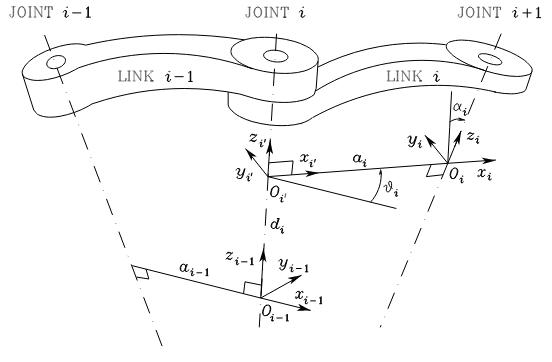
\includegraphics[scale=1]{img/DH_convention.png}
    \caption{\textbf{DH parameters}. The $z_{i}$ axis along the direction of motion for the related joint. $O_{i}$ is the intersection of ${z_i}$ with the common normal between $z_{i-1}$ and $z_{i}$, while $O_{i'}$ is the intersection between the common normal and $z_{i-1}$. $x_{i}$, ${x}_{i'}$ are chosen along the common normal from $i-1$ to $i$. The unit vectors $y_{i}$, ${y}_{i'}$ are to complete the right-handed reference frames.}
    \label{fig:DHparam}
\end{figure}

\begin{equation}
    A_i^{i-1}(q_i) = A_{i'}^{i-1} A_i^{i'} =
\begin{bmatrix}
c_{\theta_i} & -s_{\theta_i} c_{\alpha_i} & s_{\theta_i} s_{\alpha_i} & a_i c_{\theta_i} \\
s_{\theta_i} & c_{\theta_i} c_{\alpha_i} & -c_{\theta_i} s_{\alpha_i} & a_i s_{\theta_i} \\
0 & s_{\alpha_i} & c_{\alpha_i} & d_i \\
0 & 0 & 0 & 1
\end{bmatrix}
\label{eq:DH_matrix}
\end{equation}

The parameters are summarized in the \Cref{fig:DHparam} and by multiplying the matrices one can obtain the final homogeneous transformation matrix. Once the reference frames have been placed the DH parameters are defined as follows:
\begin{itemize}
    \itemsep-0.3em
    \item $a_i$ (\textit{link length}) is the distance between origins $O_i$ and $O_{i'}$; 
    \item $\alpha_i$ (\textit{link twist}) is the angle between $z_{i-1}$ and $z_{i}$ seen by the axis $x_i$ (counterclockwise to be positive)
    \item $\theta_i$ (\textit{joint angle}) is the angle between $x_{i-1}$ and $x_{i}$ seen by the axis $z_{i-1}$ (counterclockwise to be taken positive)
    \item $d_i$ (\textit{link offset}) is the coordinate of $O_{i'}$ along the axis $z_{i-1}$
\end{itemize}

\begin{remark}
    The \Cref{eq:DH_matrix} has been obtained by (post)multipliying two successive homogeneous transformation: (i) from the frame $i-1$ to $i'$; (ii) from the frame $i'$ to the frame $i$. This conceptual step of passing through the intermediate transformation can be skipped.
\end{remark}

\begin{remark}
    The reference frames to be placed are \underline{not univocally determined} in the following cases:
    \begin{itemize}
        \itemsep-0.3em
        \item With respect to the 0-th reference frame in which only the direction of the $z_0$ is determined; 
        \item With respect to the $n$-th reference frame since there is not a $n+1$ joint $z_n$ is not uniquely determined. Typically, is chosen $z_{n}\parallel z_{n-1}$; 
        \item when two consecutive axis are parallel since the common normal is not unique; 
        \item when two axis intersect in a single point, the origin is unique, while $x_i$ is arbitrary\footnote{
            Even if in order to measure an angle $x_i$ must be orthogonal to both $z_i$ and $z_{i-1}$
        }
        \item when the $i$-th joint is prismatic only the direction of $z_{i-1}$ is uniquely determined.
    \end{itemize}
    In such cases the indeterminedness can be exploited in order to simplify the procedure looking for alignment conditions between consecutive reference frames.
\end{remark}

\section{Other aspects about manipulators}

\subsection{Operational space and Joint space}
We have seen till now that the \textit{direct kinematics equation} allows to describe the position and orientation of the end-effector (the reference frame attached to it) in function of the joint variable with respect to the base reference frame. When we want to describe a task to be performed from the manipulator, we have the necessity to describe both position and orientation of $\mathcal{R_e}$ in the time (\textit{trajectories}). \\
As far as the position is concerned, we can proceed in a simple way while it is very difficult to guarantee the \textit{orthogonality condition} during the time for the end-effector unit vectors $\bb{n}_e, \bb{s}_e, \bb{n}_e$. What is useful is to reduce the rotation matrix $R_e^b$ to a minimal representation, for example the Euler angles associated to the rotation of $\mathcal{R}_e$ with respect to $\mathcal{R}_b$. In this way the end-effector pose can be expressed in terms of the following vector $\bb{x}_e$ having a number $m\le{6}$: 
\begin{equation}
    \bb{x}_e=\begin{bmatrix}
        \bb{p}_e\\
        \bb{\phi}_e
    \end{bmatrix}
\end{equation}
 where $\bb{p}_e$ is related to the position of $O_e$ while $\phi_e$ expresses the orientation of the end-effector. Such an alternative representation is more confortable: since $\bb{k}$ is a vector function, tools from calculus (derivatives, gradients...) can be used. The space in which the vector $x_e$ is defined is called \textbf{operational space} since we use it to describe the task to be performed by the manipulator. The space of the joint variables 
 \begin{equation}
    \bb{q}=\begin{bmatrix}
        q_1\\ \vdots \\ q_n
    \end{bmatrix}
 \end{equation}
is called \textbf{joint space} (or \textbf{configuration space}). We recall that 
\begin{equation}
    q_i=\begin{cases}
        d_i&\text{Prismatic joint}\\
        \theta_i&\text{Revolute joint}
    \end{cases}
\end{equation}

At this point the direct kinematic equation can be also expressed in the following form
\begin{equation}
    \bb{x}_e=\bb{k(q)}
\end{equation}
where the function $\bb{k}$ allows the computation of the operational space variables starting from the joint variables. Only in simple case finding an explicit form for $\bb{k}$ is straightforward.

\subsection{Workspace}
Taking into account the operational space, is defined \textbf{workspace} the set of points that the origin of $R_e$ can assume when the joint assume all possible configurations. Often we use to distinguish between:
\begin{itemize}
    \itemsep-0.3em
    \item \textit{Reachable workspace} is the workspace that the end effector frame can describe with at least one orientation.
    \item \textit{Dexterous workspace} is the workspace that $\mathcal{R}_e$ can reach by using many different configurations.
\end{itemize}
It appears clear that
\begin{equation*}
    \textsf{Reachable Workspace} \subseteq \textsf{Dexterous Workspace}
\end{equation*}
and points which are at the border of the workspace are reachable by uing a single orientation.

\subsection{Accuracy and Repeteability}
\subsubsection{Accuracy}
In a real manipulator there is always a discrepance between computed and real DH parameters, this is essentially due to mechanical tolerances. Since DH parameters are used in order to obtain the direct kinematics equation, the effective pose the manipulator attain with respect to the computed one by using the homogeneous transformation matrix $\bb{T}_e^b$. The \textit{discrepancy} between real and computed solution is called \textbf{accuracy}. Modern manipulators guarantee an accuracy of the order of 1mm. In order to have a good accuracy, it is need a sufficiently rigid structure of the shoulder.

\subsubsection{Repeteability}
Refers to the ability of the manipulators to return to a previously reached position. It depends on the mechanical structure, on the sensors/transducers (especially from the resolution) and on the control strategies which are used, it is smaller than the accuracy. 
Modern manipulators have, even better performances with respect to the repeteability.

\section{The \textit{Inverse Kinematics} problem} 
The \textbf{inverse kinematics problem} is related to finding what is $\bb{q}$ (joint variables) which gives a certain end-effector position and orientation $\bb{x}_e$. This is not a simple problem since: (i) closed form solutions could not exist; (ii) multiple or infinite solutions could exist; (iii) there are cases in which no solutions are available. There is a nice property which guarantee the existence of a solution if $\bb{x}_e$ belongs to the dexterous workspace. \\
The \textit{inverse kinmeatic problem} could be solved by using algebraic or geometrical intuitions. In the former case we have to solve nonlinear trascendent equations, in the latter case we are looking for significant points which lead to the provided position and orientation of the end-effector. Very often \textbf{numerical methods} are used in order to find a valid configuration for which a certain pose of the end-effector is attained. 

{\Large
\begin{equation}
    \text{given } \ \bb{x}_e(\bb{q}) \to \text{I want } \bb{q} 
\end{equation}
}
\chapter{Differential Kinematics of manipulators}

%Appendices
\appendix
\renewcommand{\thechapter}{\Alph{chapter}}
\renewcommand{\theHchapter}{\thechapter}
\setcounter{chapter}{0}
%\chapter{Linear algebra notions \colorbox{yellow}{\texttt{TO DO...}}}
\section{Gradient and Jacobian}
\section{Matrix operations}
\section{Vector product}
\section{Bilinear form and quadratic form}
%\chapter{Rigib body mechanics \colorbox{yellow}{\texttt{TO DO...}}}
\section{Dynamics}
\section{Energy and Work}
\section{Multibody system mechanics}

\printbibliography


\end{document}